\documentclass{article}

\usepackage[T2A]{fontenc}
\usepackage[utf8]{luainputenc}
\usepackage[english, russian]{babel}
\usepackage[pdftex]{hyperref}
\usepackage[14pt]{extsizes}
\usepackage{listings}
\usepackage{color}
\usepackage{geometry}
\usepackage{enumitem}
\usepackage{multirow}
\usepackage{graphicx}
\usepackage{indentfirst}
\usepackage[ruled,vlined,linesnumbered]{algorithm2e}

\newenvironment{myalgorithm}[1][htb]
  {\renewcommand{\algorithmcfname}{Алгоритм}
   \begin{algorithm}[#1]%
  }{\end{algorithm}}

\setlength{\parskip}{3mm}
\geometry{a4paper,top=20mm,bottom=20mm,left=25mm,right=15mm}
\setlist{nolistsep, itemsep=0.5cm,parsep=0pt}

\usepackage{xcolor}

\colorlet{mygray}{black!30}
\colorlet{mygreen}{green!60!blue}
\colorlet{mymauve}{red!60!blue}
\colorlet{myred}{red!60!blue}

\lstset{
  backgroundcolor=\color{gray!10},  
  basicstyle=\fontsize{13}{13}\ttfamily,
  columns=fullflexible,
  breakatwhitespace=false,      
  breaklines=true,                           
  commentstyle=\color{mygreen},                      
  keepspaces=true,             
  keywordstyle=\color{blue},      
  language=c++,                 
  numbers=none,                
  numbersep=1pt,                   
  numberstyle=\tiny\color{blue}, 
  rulecolor=\color{mygray},        
  showspaces=false,               
  showtabs=false,                                  
  stringstyle=\color{mymauve},                         
  title=\lstname                
}

\makeatletter
\renewcommand\@biblabel[1]{#1.\hfil}
\makeatother

\begin{document}

\begin{titlepage}

\begin{center}
Министерство науки и высшего образования Российской Федерации \\
\vspace{5mm}
Федеральное государственное автономное образовательное учреждение высшего образования \\
Национальный исследовательский Нижегородский государственный университет им. Н.И. Лобачевского \\
\vspace{1cm}
Институт информационных технологий, математики и механики \\
\vspace{5cm}
\textbf{\large Отчет по лабораторной работе} \\
\vspace{8mm}
\textbf{\Large «Построение выпуклой оболочки - проход Джарвиса»} \\
\end{center}

\vspace{3cm}

\newbox{\lbox}
\savebox{\lbox}{\hbox{text}}
\newlength{\maxl}
\setlength{\maxl}{\wd\lbox}
\hfill\parbox{7cm}{
\hspace*{5cm}\hspace*{-5cm}\textbf{Выполнила:} \\ студент группы 381706-2 \\ Ясакова А. Е.\\
\\
\hspace*{5cm}\hspace*{-5cm}\textbf{Проверил:}\\ доцент кафедры МОСТ, \\ кандидат технических наук \\ Сысоев А. В.
}

\vspace{\fill}

\begin{center} 
Нижний Новгород \\ 2020
\end{center}
\end{titlepage}

\setcounter{page}{2}

\tableofcontents

\newpage

\section{Введение}
Вычислительная геометрия занимается изучением разработки и исследования алгоритмов для решения геометрических проблем. Задача построения выпуклых оболочек, является одной из центральных задач вычислительной геометрии. Важность этой задачи происходит не только из-за огромного количества приложений (в распознавании образов, обработке изображений, базах данных, в задаче раскроя и компоновки материалов, математической статистике), но также и из-за полезности выпуклой оболочки как инструмента решения множества задач вычислительной геометрии.

\par Для практических целей выпуклые оболочки полезны тем, что они компактно хранят всю необходимую информацию о множестве точек, что позволяет быстро отвечать на разнообразные запросы на этом множестве.

\par Выпуклые оболочки очень важны в ряде геометрических положений не только сами по себе, но и как части других алгоритмов, использующих построение выпуклой оболочки в качестве элементарной операции.

\par Джарвис обратил внимание на то, что многоугольник, которым является выпуклая оболочка, с одинаковым успехом можно задать упорядоченным множеством как его ребер, так и его вершин. Если задано множество точек, то довольно трудно быстро определить, является или нет некоторая точка крайней. Однако, если даны две точки, то непосредственно можно проверить, является или нет соединяющий их отрезок ребром выпулой оболочки.

\newpage

\section{Постановка задачи}

В рамках лабораторной работы нужно реализовать алгоритм построения выпуклой оболочки - проход Джарвиса.

\par Требуется выполнить следующее:

\begin{enumerate}
\item Изучить и реализовать последовательный алгоритм Джарвиса.
\item Разработать и реализовать параллельный алгоритм Джарвиса с использованием технологий OpenMP, TBB и std::threads.
\item Довести до успешного выполнения тесты, созданные с использованием Google C++ Testing Framework.
\item Провести вычислительные эксперименты и сделать выводы, почему получились именно такие результаты.
\end{enumerate}

\newpage

\section{Метод решения}

Выпуклой оболочкой множества точек S называется наименьшее выпуклое множество, содержащее S.

\par Выберем какую-нибудь точку $p_{0}$, которая гарантированно попадёт в выпуклую оболочку. Например, нижнюю, а если таких несколько, то самую левую из них.

\par Дальше будем действовать так: найдём самую «правую» точку от последней добавленной (то есть точку с минимальным полярным углом) и добавим её в оболочку. Будем так итеративно добавлять точки, пока не «замкнёмся», то есть пока самой правой точкой не станет $p_{0}$.

\begin{figure}[h]
\centering
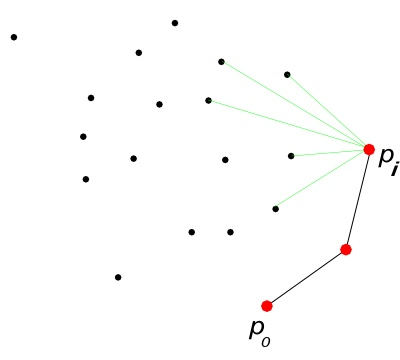
\includegraphics[scale=1.1]{../../../../modules/reports/yasakova_a_jarvis_alg/picture.png}
\caption{Иллюстрация алгоритма}
\end{figure}

\begin{myalgorithm}[H]
\SetAlgoLined
\BlankLine
$p[1] = the\:lower\:left\:point\:P$\;
$p[2] =minimum\:positive\:polar\:angle\:from\:p[1]$\;
$i = 2$\;
\BlankLine
\While{p[i] != p[1]} {
	\For{j от 1 до |P|}{
		$p[i+1] = min\:cos(p[i-1],\:p[i],\:P[j])$\;
	}
	$i = i + 1$\;
}
$return\:p$\;
\caption{Построение выпуклой оболочки - проход Джарвиса}
\end{myalgorithm}

\par Для каждой точки выпуклой оболочки (обозначим их количество за h) мы из всех оставшихся O(n) точек будем искать оптимальную, что суммарно будет работать за O(n*h).


\newpage

\section{Схема распараллеливания}

Рассмотрим реализацию алгоритма Джарвиса с точки зрения задачи параллелизации вычислений.

\par Рассмотрим реализацию поэтапно.

\par Первым делом распараллеливаем поиск первой и второй точек - два цикла по всем точкам.

\par Далее идет внешний цикл, который заканчивается, когда находим всю выпуклую оболочку, внутри цикл по всем точкам. Есть несколько вариантов распараллеливания. Первый способ - поделить точки между потоками и найти выпуклые оболочки для каждого из этих множеств. В результате, у каждого потока будет своя выпуклая оболочка. Далее следует найти результирующую выпулую оболочку на получившемся множестве. Второй способ - распараллелить внутренний цикл по всем точкам. Первый вариант лучше, так как внутри внешнего цикла каждый раз не создаются потоки для работы. Но с другой стороны, второй вариант не делает лишней работы, обходя одни и те же точки по два раза, как делает первый. Первым способом я реализовала данный алгоритм на основе библиотеки TBB. Вторым способом была выполнена программа с помощью OpenMP и std::thread.

\newpage

\section{Описание программной реализации}
Множество точек в программе выглядит как вектор пар значений - {($x_{1}$, $y_{1}$), ($x_{2}$, $y_{2}$), ..., ($x_{n}$, $y_{n}$)}.

\begin{lstlisting}
	std::vector<std::pair<int, int>> points;
\end{lstlisting}

\par В программе реализованы следующие методы:

\begin{lstlisting}
	std::vector <std::pair<int, int>> GetRandomPoints(int n);
\end{lstlisting}

- случайный подбор множества чисел;

\begin{lstlisting}
	std::vector < std::pair<int, int>> JarvisAlg(cons std::vector<std::pair<int, int>>& points);
\end{lstlisting}

- алгоритм Джарвиса, включает в себя вызов следующих двух функций и цикл, пока не найдем выпуклую оболочку;

\begin{lstlisting}
	std::pair<int, int> FindFirstPoint(const std::vector<std::pair<int, int>>& points);
\end{lstlisting}

- поиск первой точки - левая из самых нижних;

\begin{lstlisting}
	std::pair<int, int> FindSecondPoint(const std::vector<std::pair<int, int>>& points, std::pair<int, int> tmp);
\end{lstlisting}

- поиск второй точки - наименьший полярный угол;

\begin{lstlisting}
	double CountCos(std::pair<int, int> a, std::pair<int, int> b, std::pair<int, int> c);
\end{lstlisting}

- подсчет косинуса угла, составленного этими точками;

\begin{lstlisting}
	double distance(std::pair<int, int> a, std::pair<int, int> b);
\end{lstlisting}

- определение расстояния между двумя точками.

\newpage

\section{Подтверждение корректности}
Для подтверждения корректности в программе реализован набор тестов с использованием библиотеки для модульного тестирования Google C++ Testing Framework. Тесты проверяют корректную работу последовательного и параллельных алгоритмов.

\par Дополнительно для подтверждения корректности в программе реализована демонстрация работы алгоритма визуально с использованием библиотеки OpenCV.

\subsection{Список тестов}

Рассмотрим тесты на примере реализации параллельного алгоритма с помощью технологии OpenMP (программы, написанные с помощью технологий TBB и std::thread, имеют аналогичные тесты).

\begin{itemize}
\item TEST(OpenMP\_Test, test1) - исходное множество содержит три точки, все точки являются выпуклой оболочкой;
\item TEST(OpenMP\_Test, test2) - исходное множество содержит вершины некоторого квадрата и несколько точек внутри этого квадрата, вершины квадрата являются выпуклой оболочкой;
\item TEST(OpenMP\_Test, test3) - две точки находятся на одной прямой, в выпуклую оболочку берется дальняя;
\item TEST(OpenMP\_Test, test4) - произвольные точки;
\item TEST(OpenMP\_Test, test5) - произвольные точки;
\item TEST(OpenMP\_Test, test6) - сравнение результатов последовательного и параллельного алгоритмов.
\end{itemize}

\newpage

\section{Результаты экспериментов}
Характеристики ПK:

\begin{itemize}
\item Процессор: Intel® Core™ i5-85250U CPU @ 1.60GHz 1.80 GHz
\item Оперативная память: 8,00 ГБ
\item Операционная система: Windows 10
\item Число ядер: 4.
\end{itemize}


\par Для проведения экспериментов задействовано 4 потока. Сложность данного алгоритма - O(n*m), где n - общее количество точек в исходном множестве точек, а m - количество точек в получившейся выпуклой оболочке. Общее число точек в экспериментах равно 100000000. Замеры времени осуществлялись только тогда, когда количество точек в выпулой оболочке было одинаковое (равно 8). Результаты экспериментов приведены в таблице 1.

\begin{table}[!h]
\centering
\begin{tabular}{|c|c|c|c|c|c|c|c|}
\hline
\multirow{2}{*}
{\begin{tabular}[c]{@{}c@{}}Последовательный\\ алгоритм\end{tabular}} &
\multicolumn{6}{c|}
{Параллельный алгоритм} \\
\cline{2-7} &
\multicolumn{2}{c|}{OpenMP} &
\multicolumn{2}{c|}{TBB} &
\multicolumn{2}{c|}{std::thread}
\\ \cline{1-7}
t, с  & t, с & speedup & t, с & speedup & t, с & speedup \\ \hline
13.58 & 5.66 & 2.4     & 5.92 & 2.29    & 4.38 & 3.1 \\ \hline
\end{tabular}
\caption{Средние значения результатов экспериментов}
\end{table}

\par В экспериментах осуществлялся замер времени выполнения алгоритма Джарвиса и высчитывалось ускорение программы путем деления времени исполнения последовательного алгоритма на время параллельного.

\par По полученным результатам можно заметить, что параллельный алгоритм с использованием технологии std::thread имеет самое лучшее ускорение. Самое маленькое ускорение оказалось у TBB, так как эта технология имеет много функционала, следовательно, большее время обработки: создание среды для работы потоков, создание самих потоков и распределение задач между потоками.


\newpage

\section{Заключение}
В ходе выполнения данной работы все поставленные цели были достигнуты, а именно подробно изучен алгоритм построения выпулой оболочки - проход Джарвиса, разработана реализация эффективной параллельной версии алгоритма с использованием технологий: OpenMP, TBB, std::threads, разработаны и доведены до успешного выполнения тесты, созданные с использованием Google C++ Testing Framework, выполнены замеры времени, по которым было определено, что лучшей технологией для реализации параллельного алгоритма Джарвиса оказалась технология std::thread.

\par В заключении нужно отметить, что алгоритм Джарвиса является достаточно простым в понимании и реализации. Его сложность O(n*m), где n - общее количество точек в исходном множестве точек, а m - количество точек в получившейся выпуклой оболочке, что в общем случае дает хороший результат по времени выполнения.
\newpage

\section{Список литературы}
Книги:

\begin{itemize}
\item Гергель В.П. Учебный курс «Введение в методы параллельного программирования», раздел «Параллельное программирование с использованием OpenMP». Нижний Новгород, ННГУ, 2007, 33 с.
\item А.А. Сиднев, А.В. Сысоев, И.Б. Мееров. Учебный курс «Технологии разработки параллельных программ», раздел «Создание параллельной программы», «Библиотека Intel Threading Building Blocks~-— краткое описание». Нижний Новгород, ННГУ, 2007, 29 с.
\end{itemize}

\par Интернет-ресурсы:

\begin{itemize}
\item Выпуклые оболочки \\ URL: https://algorithmica.org/ru/convex-hulls
\item std::thread \\ URL: https://en.cppreference.com/w/cpp/thread/thread
\end{itemize}

\newpage

\section{Приложение}
\subsection{Последовательный алгоритм Дейкстры}
\lstinputlisting[language=C++, caption=Заголовочный файл]{../../../../modules/task_1/yasakova_a_jarvis_alg/jarvis_alg.h}
\lstinputlisting[language=C++, caption=Cpp файл]{../../../../modules/task_1/yasakova_a_jarvis_alg/jarvis_alg.cpp}
\lstinputlisting[language=C++, caption=Тесты]{../../../../modules/task_1/yasakova_a_jarvis_alg/main.cpp}

\subsection{OpenMP}
\lstinputlisting[language=C++, caption=Заголовочный файл]{../../../../modules/task_2/yasakova_a_jarvis_alg/jarvis_alg.h}
\lstinputlisting[language=C++, caption=Cpp файл]{../../../../modules/task_2/yasakova_a_jarvis_alg/jarvis_alg.cpp}
\lstinputlisting[language=C++, caption=Тесты]{../../../../modules/task_2/yasakova_a_jarvis_alg/main.cpp}

\subsection{TBB}
\lstinputlisting[language=C++, caption=Заголовочный файл]{../../../../modules/task_3/yasakova_a_jarvis_alg/jarvis_alg.h}
\lstinputlisting[language=C++, caption=Cpp файл]{../../../../modules/task_3/yasakova_a_jarvis_alg/jarvis_alg.cpp}
\lstinputlisting[language=C++, caption=Тесты]{../../../../modules/task_3/yasakova_a_jarvis_alg/main.cpp}

\subsection{std::thread}
\lstinputlisting[language=C++, caption=Заголовочный файл]{../../../../modules/task_4/yasakova_a_jarvis_alg/jarvis_alg.h}
\lstinputlisting[language=C++, caption=Cpp файл]{../../../../modules/task_4/yasakova_a_jarvis_alg/jarvis_alg.cpp}
\lstinputlisting[language=C++, caption=Тесты]{../../../../modules/task_4/yasakova_a_jarvis_alg/main.cpp}



\end{document}